\subsection{Layer Summaries}

\begin{figure}[b]
\centering
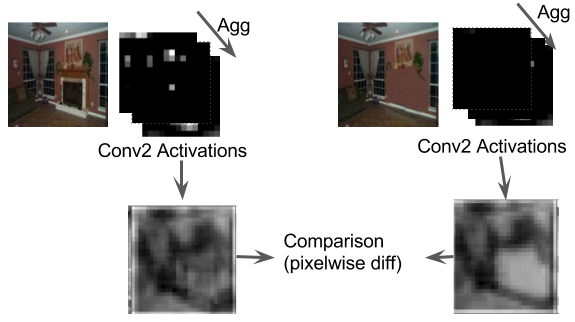
\includegraphics[width=\columnwidth]{figures/layer_summary_fig}
\caption{Generation of Layer Summaries for Comparison with Perturbed Images}

\label{fig:act_im_summary_fig}
\end{figure}

We define a layer summary as an pixel by pixel aggregation over the activations images in a layer of a CNN. For instance, the conv4 layer of Alexnet~\cite{alexnet} contains 256 distinct $14 \times 14$ activation images. We generate an layer summary by aggregating over each pixel across the set of activation images in a layer. Layer summaries are useful for comparing the activations of an image and a perturbed version of the image as in Figure ~\ref{fig:act_im_summary_fig}. We hypothesize that for a perturbed image, where the change in the image does not cause a change in the output class, that the impacts of the change should become less apparent the the summary images of deeper layers of a well behaved network. In a poorly performing network, however, the change will be visible in the summary images of deeper layers.

Different aggregation functions reveal different properties of a set of activation images. For instance, an average has a contribution from all of the input images, but makes it difficult to detect large changes in a single activation image. Whereas, a maximum over the images is sensitive to the changes in a single activation and is unable to detect changes that occur over large sets of activations. We explore the trade-offs of the choice of aggregation in section \todo{add ref to relevant section}.